
\part{Principes généraux}

\section{Jeu au tour par tour}

Batailles Fantastiques : Le 9\ieme{} Âge est un jeu au tour par tour. Une partie ordinaire se joue en 6 Tours de Jeu. Un Tour de Jeu se décompose en deux Tours de Joueur. Un joueur a le premier Tour de Joueur, pendant lequel il déplace ses figurines et attaque avec elles. Après cela, l'autre joueur joue son premier Tour de Joueur, ce qui finit le premier Tour de Jeu. Durant le deuxième Tour de Jeu, le premier joueur joue maintenant son deuxième Tour de Joueur, et ainsi de suite, jusqu'à ce que les deux joueurs aient fait six Tours de Joueur, ce qui termine la partie.

\subsection{Tour de Joueur}

Chaque Tour de Joueur se divise en quatre Phases jouées dans l'ordre suivant :

\hspace*{0.3cm}
\begin{tabular}{c|l}
1 & Phase de Mouvement \tabularnewline
2 & Phase de Magie \tabularnewline
3 & Phase de Tir \tabularnewline
4 & Phase de Corps à Corps \tabularnewline
\end{tabular}

\subsection{Joueur Actif et Joueur Réactif}

Le Joueur Actif est le joueur qui est en train de jouer son tour.

Le Joueur Réactif est le joueur qui n'est pas en train de jouer son tour.

\subsection{Effets simultanés}

\newfromWHB{À chaque fois qu'au moins deux effets sont activés en même temps, et que leur ordre importe, commencez par résoudre tous les effets contrôlés par le Joueur Actif. Chaque joueur décide de l'ordre dans lequel ses propres effets sont résolus. Si une décision est nécessaire, par exemple pour activer ou non une capacité, le Joueur Actif doit déclarer ses choix avant le Joueur Réactif. Une fois que les deux joueurs ont déclaré quelles capacités sont activées et dans quel ordre, les effets sont résolus, en commençant par le Joueur Actif.} Par exemple, si les deux joueurs ont une capacité qui peut être activée au début de la Phase de Magie, le joueur dont c'est la Phase de Magie doit décider en premier s'il utilise sa capacité ou non. Ensuite, le Joueur Réactif peut choisir s'il utilise la sienne. Enfin, les effets sont résolus, en commençant par la capacité du Joueur Actif.

\newpage
\section{Les dés}

\subsection{Lancer les dés}

Dans Batailles Fantastiques : Le 9\ieme{} Âge, on utilise souvent des dés pour déterminer ce qu'il s'y passe. Le dé le plus utilisé est un dé à six faces, appelé \og D6 \fg{}, dont les valeurs vont de 1 à 6. Un jet de dé est généralement réussi si le résultat est supérieur ou égal à une certaine valeur, par exemple si le dé donne \result{3} ou plus. Cela est indiqué par un \og 3+ \fg{} (ou 2+, 4+, 6+, etc.). Vous devez quelquefois lancer plusieurs de ces dés en même temps. Cela est représenté par un nombre avant le type de dé, comme \og 3D6 \fg{}, qui signifie qu'il faut lancer 3 dés à six faces et additionner leurs résultats. Dans d'autres cas, un jet de dé peut être modifié par addition ou soustraction d'un chiffre, comme \og 1D6+1 \fg{}. Ajoutez ou soustrayez le chiffre indiqué au résultat du dé. Enfin, certains effets permettent de relancer des dés, comme des jets pour blesser ratés, ou des jets de Sauvegarde Invulnérable ayant donné \result{1}. Relancez simplement le ou les dés en question.

\textbf{Un dé relancé ne peut jamais être relancé à nouveau}, peu importe la raison ou la capacité, et le second résultat doit toujours être accepté.

Il est parfois nécessaire de lancer un D3. Il suffit de lancer un D6 et de diviser le résultat par deux, en arrondissant au supérieur, pour un résultat de 1, 2 ou 3. Quand on parle d'un résultat naturel de \result{1} ou \result{6} à propos d'un jet de D3, on fait toujours référence au résultat du D6 avant la division par deux.

\subsection{Le dé de déviation}

Le Dé de Déviation est un dé à six faces spécial. Deux de ses faces sont marquées d'un symbole \og Touché ! \fg{} et les quatre autres faces d'une flèche, pointant ainsi dans une direction aléatoire. Ce dé est généralement utilisé quand un projectile ou l'effet d'un sort risque de dévier de sa trajectoire.

\begin{figure}[!htbp]
\begin{minipage}{0.3\textwidth}
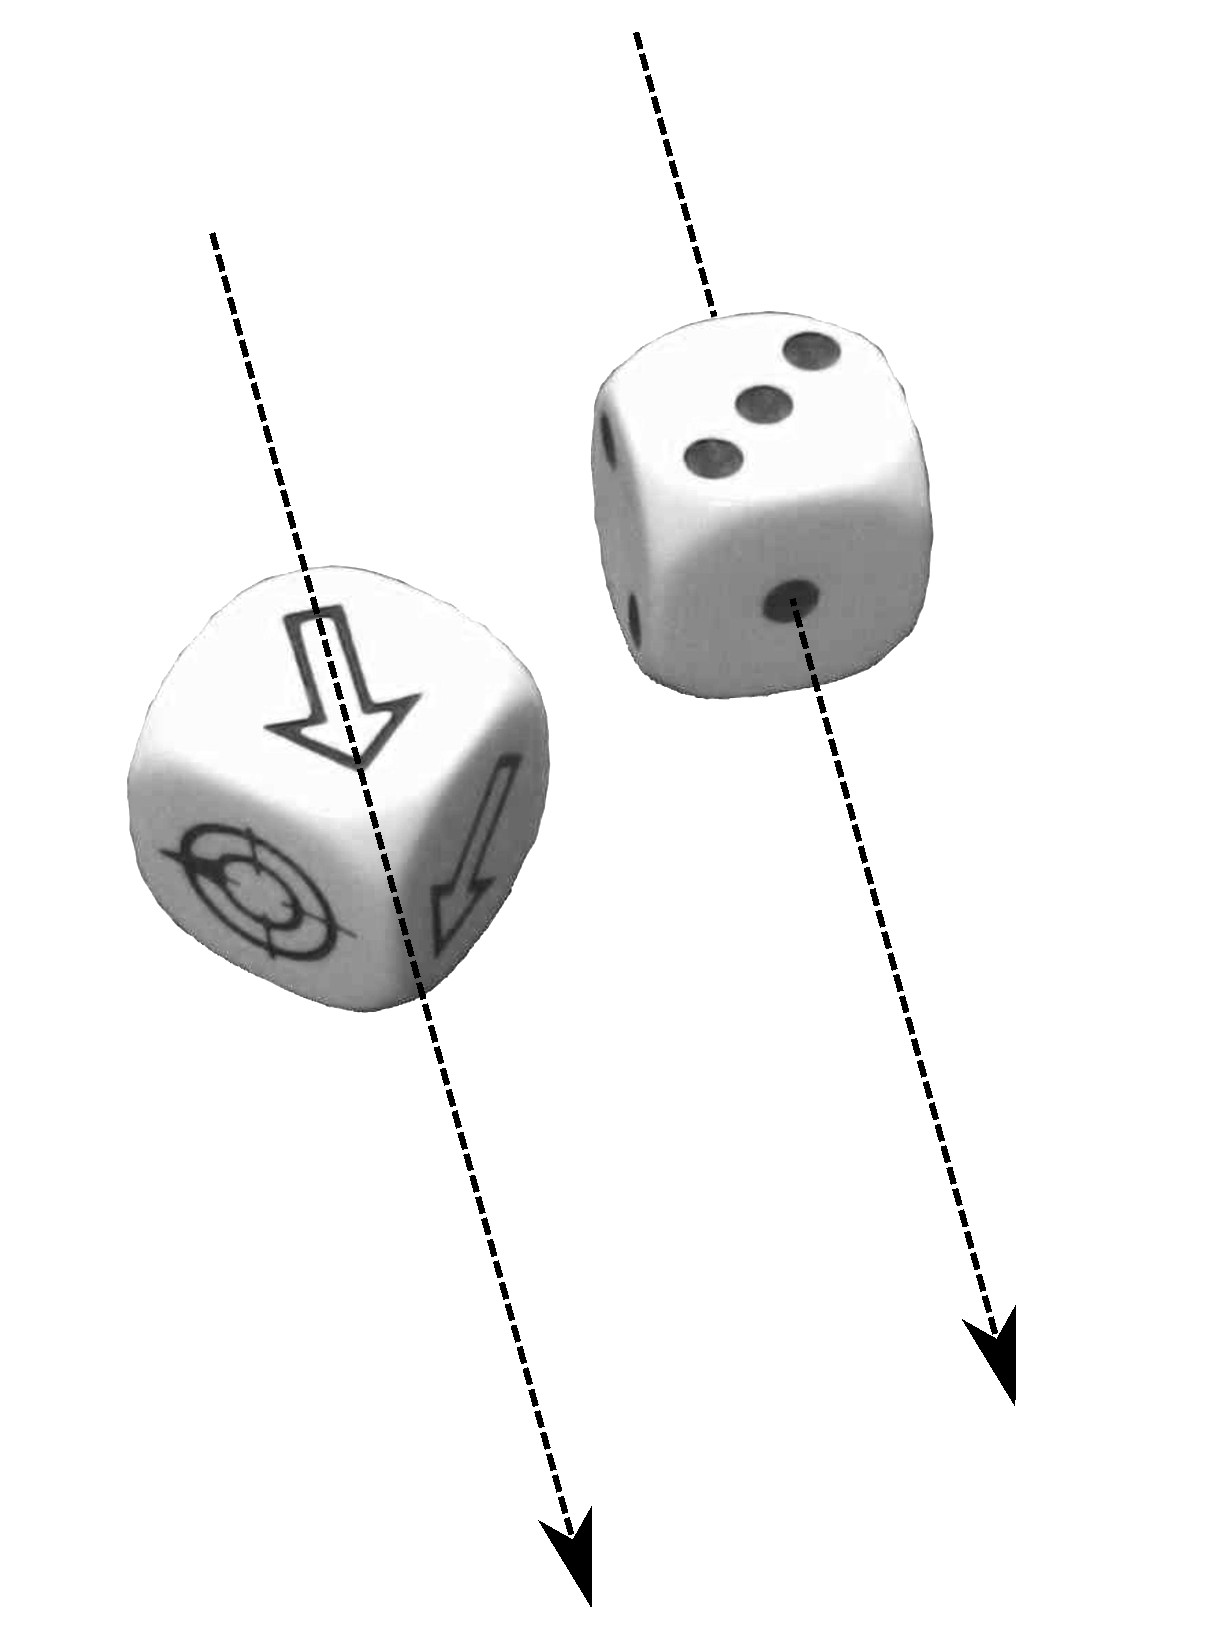
\includegraphics[width=\textwidth]{pics/deviation_dice.png}
\caption{Deux façons équivalentes de représenter un Dé de Déviation.}
\label{figure/deviation_dice}
\end{minipage}\hfill
\begin{minipage}{0.67\textwidth}
\paragraph{Déviation}

Quand vous êtes amenés à faire dévier un objet, par exemple avec \og Faites dévier le gabarit de \distance{1D6} \fg{}, lancez le Dé de Déviation. Si un symbole \og Touché ! \fg{} est obtenu, ne bougez pas l'objet. Si une flèche est obtenue, déplacez le gabarit de la distance indiquée dans la description de la règle parallèlement à la direction de la flèche. Notez qu'il ne s'agit pas de la même chose que de déterminer une direction aléatoire.

\vspace*{3ex}
\paragraph{\newfromWHB{Utiliser un dé classique à la place}}

Un dé à six faces ordinaire peut faire l'affaire pour remplacer un Dé de Déviation. Un résultat de \result{1} ou \result{6} représente un \og Touché ! \fg . Sinon, le symbole \result{1} pointe une direction comme une flèche (voir la figure \ref{figure/deviation_dice}).
\end{minipage}
\end{figure}

\subsection{Direction aléatoire}

Dans certains cas, vous devrez déterminer une direction aléatoire. Lancez alors le Dé de Déviation jusqu'à obtenir une flèche et utilisez cette direction. Ignorez tout résultat \og Touché ! \fg{}. Vous pouvez exceptionnellement relancer ce dé plusieurs fois jusqu'à obtenir une flèche. Certains Dés de Déviation disposent d'une petite flèche sur le symbole \og Touché ! \fg{}. Il est donc inutile de relancer ce dé, utilisez la petite flèche pour la direction.

\section{Gabarits}

Les Gabarits sont utilisés pour déterminer des zones d'effet. Il y en a de différents types et tailles, les plus employés étant les Gabarits de \distance{3} et \distance{5}. Ces derniers ont une forme de disque, de diamètres respectifs \distance{3} et \distance{5}. Les Gabarits moins communs comprennent le Gabarit rond de \distance{1}, appelé simplement Gabarit de \distance{1}, et le Gabarit Linéaire, utilisé pour les canons et certains sorts.

Pour définir combien de figurines sont touchées par un Gabarit (on dit aussi sous un Gabarit), tenez le Gabarit en question au-dessus de la cible et déterminez quelles figurines ont leur socle directement en dessous. Si n'importe quelle partie du socle d'une figurine, aussi petite soit-elle, est recouverte par le Gabarit, la figurine compte comme étant touchée. Un point du Gabarit ne peut toucher qu'un socle au plus. Notez que les dimensions des socles des figurines sont dans une base métrique alors que les tailles des Gabarits s'expriment en pouces. Cela signifie par exemple qu'un Gabarit de \distance{3} peut toucher les socles de 5 figurines alignées ayant des socles de \unit{25}{\milli\meter}, car \distance{3} = 7,62 {\centi\meter}.

\subsection{Touches des Gabarits circulaires}

La figure \ref{figure/templates} et la table \ref{table/templates_hits} présentent le nombre de figurines qui peuvent être touchées pour chacun des deux Gabarits circulaires.


\begin{figure}[!htbp]
\centering
\vspace*{0.3cm}
\def\svgwidth{\textwidth}
\input{pics/Templates.pdf_tex}
\caption{Placement optimal des Gabarits circulaires. Les socles verts font \unit{20x20}{\milli\meter}, les socles magenta \unit{25x25}{\milli\meter}, les socles cyan \unit{40x40}{\milli\meter} et les socles oranges \unit{25x50}{\milli\meter}.}
\label{figure/templates}
\end{figure}

\begin{table}[!htbp]
\centering
\vspace*{0.2cm}
\begin{tabular}{M{2.5cm}M{2.5cm}M{2.5cm}M{2.5cm}M{2.5cm}}
\hline
Taille de socle & \unit{20x20}{\milli\meter} & \unit{25x25}{\milli\meter} & \unit{40x40}{\milli\meter} & \unit{25x50}{\milli\meter} \tabularnewline
Gabarit de \distance{3} & 22 & 16 & 9 & 11 \tabularnewline
Gabarit de \distance{5} & 48 & 34 & 16 & 24 \tabularnewline
\hline
\end{tabular}
\caption{Nombre maximal de figurines touchées.}
\label{table/templates_hits}
\end{table}


\subsection{\linetemplate}

Un \linetemplate{} est une ligne droite tracée entre deux points. \newfromWHB{Toutes les figurines dont le socle se situe sous la ligne sont touchées.} On peut aussi déterminer le nombre de figurines touchées en additionnant le nombre de rangs et de colonnes traversés et en retirant un. Dans la figure \ref{figure/linetemplate}, 4 rangs et 4 colonnes sont traversés, soit 4 + 4 - 1 = 7 figurines touchées.

\begin{figure}[!htbp]
\centering
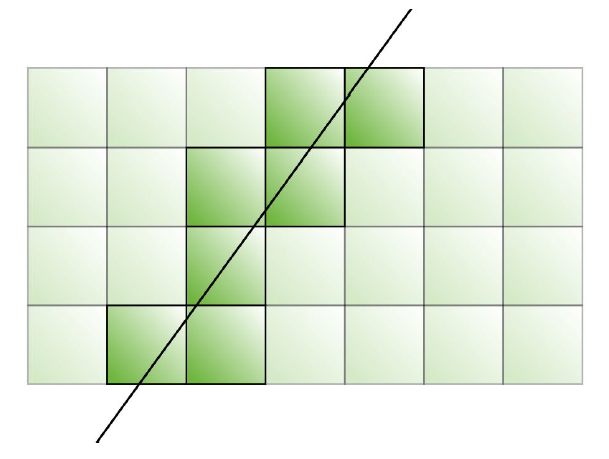
\includegraphics[width=7cm]{pics/linetemplate.png}
\caption{Touches d'un \linetemplate{}.}
\label{figure/linetemplate}
\end{figure}
